\chapter{Umsetzung und Evaluation des optimierten Prozesses}

%-> Konkrete Umsetzung/ Ausgestaltung des optimierten Prozesses im System 

%-> Generelles Ziel SAP-Consulting: Immer Standard, wenn irgendwie möglich

\section{Lösung 1: Anpassung des Standards}

-> Abbildung des Prozesses im System bei Beschränkung auf Anpassung des Standards innerhalb der Customizing Grenzen

\section{Lösung 2: Entwicklung einer kundenspezifischen Lösung}

Die zweite Möglichkeit die Kundenanforderungen umzusetzen ist die Entwicklung einer kundenspezifischen Lösung. Allgemein bietet sich im konkreten Fall die Entwicklung einer Fiori-App an, über die die Daten im System gepflegt werden können. SAP Fiori ist ein Framework für die Entwicklung und Bereitstellung von SAP-Apps. Durch ein einheitliches und rollenbasiertes Layout entsteht eine intuitiv bedienbare und konsistente Benutzeroberfläche. Da Fiori Apps responsive sind, können diese auf verschiedenen Endgeräten genutzt werden, um die Produktivität der Nutzer zu steigern. Insgesamt soll Fiori die UX von SAP-Anwendungen, vor allem für unerfahrenere Nutzer, verbessern.\footcite[Vgl.][]{praxis_sap_fiori_allgemein_2024} Fiori bietet mehrere Vorlagen an, die als Basis für die Entwicklung einer App genutzt werden können. Für den betrachteten Prozess bietet sich der ''Wizard-Floorplan'' an, da dieser eine schrittweise Benutzerführung durch mehrstufige Prozesse bietet. So können komplexe Aufgaben in kleinere Schritte unterteilt werden zwischen denen der Benutzer navigieren kann und bei denen er bei Bedarf Hilfestellungen und Fehlermeldungen erhält. So soll die UX gesteigert und die Fehlerquote gesenkt werden \parencite[Vgl.][]{praxis_sap_wizard_floorplan_2024}. Im Folgenden soll dieser Floorplan anhand des ersten Prozessschrittes exemplarisch beschrieben werden.

\begin{figure}[H]
    \centering
    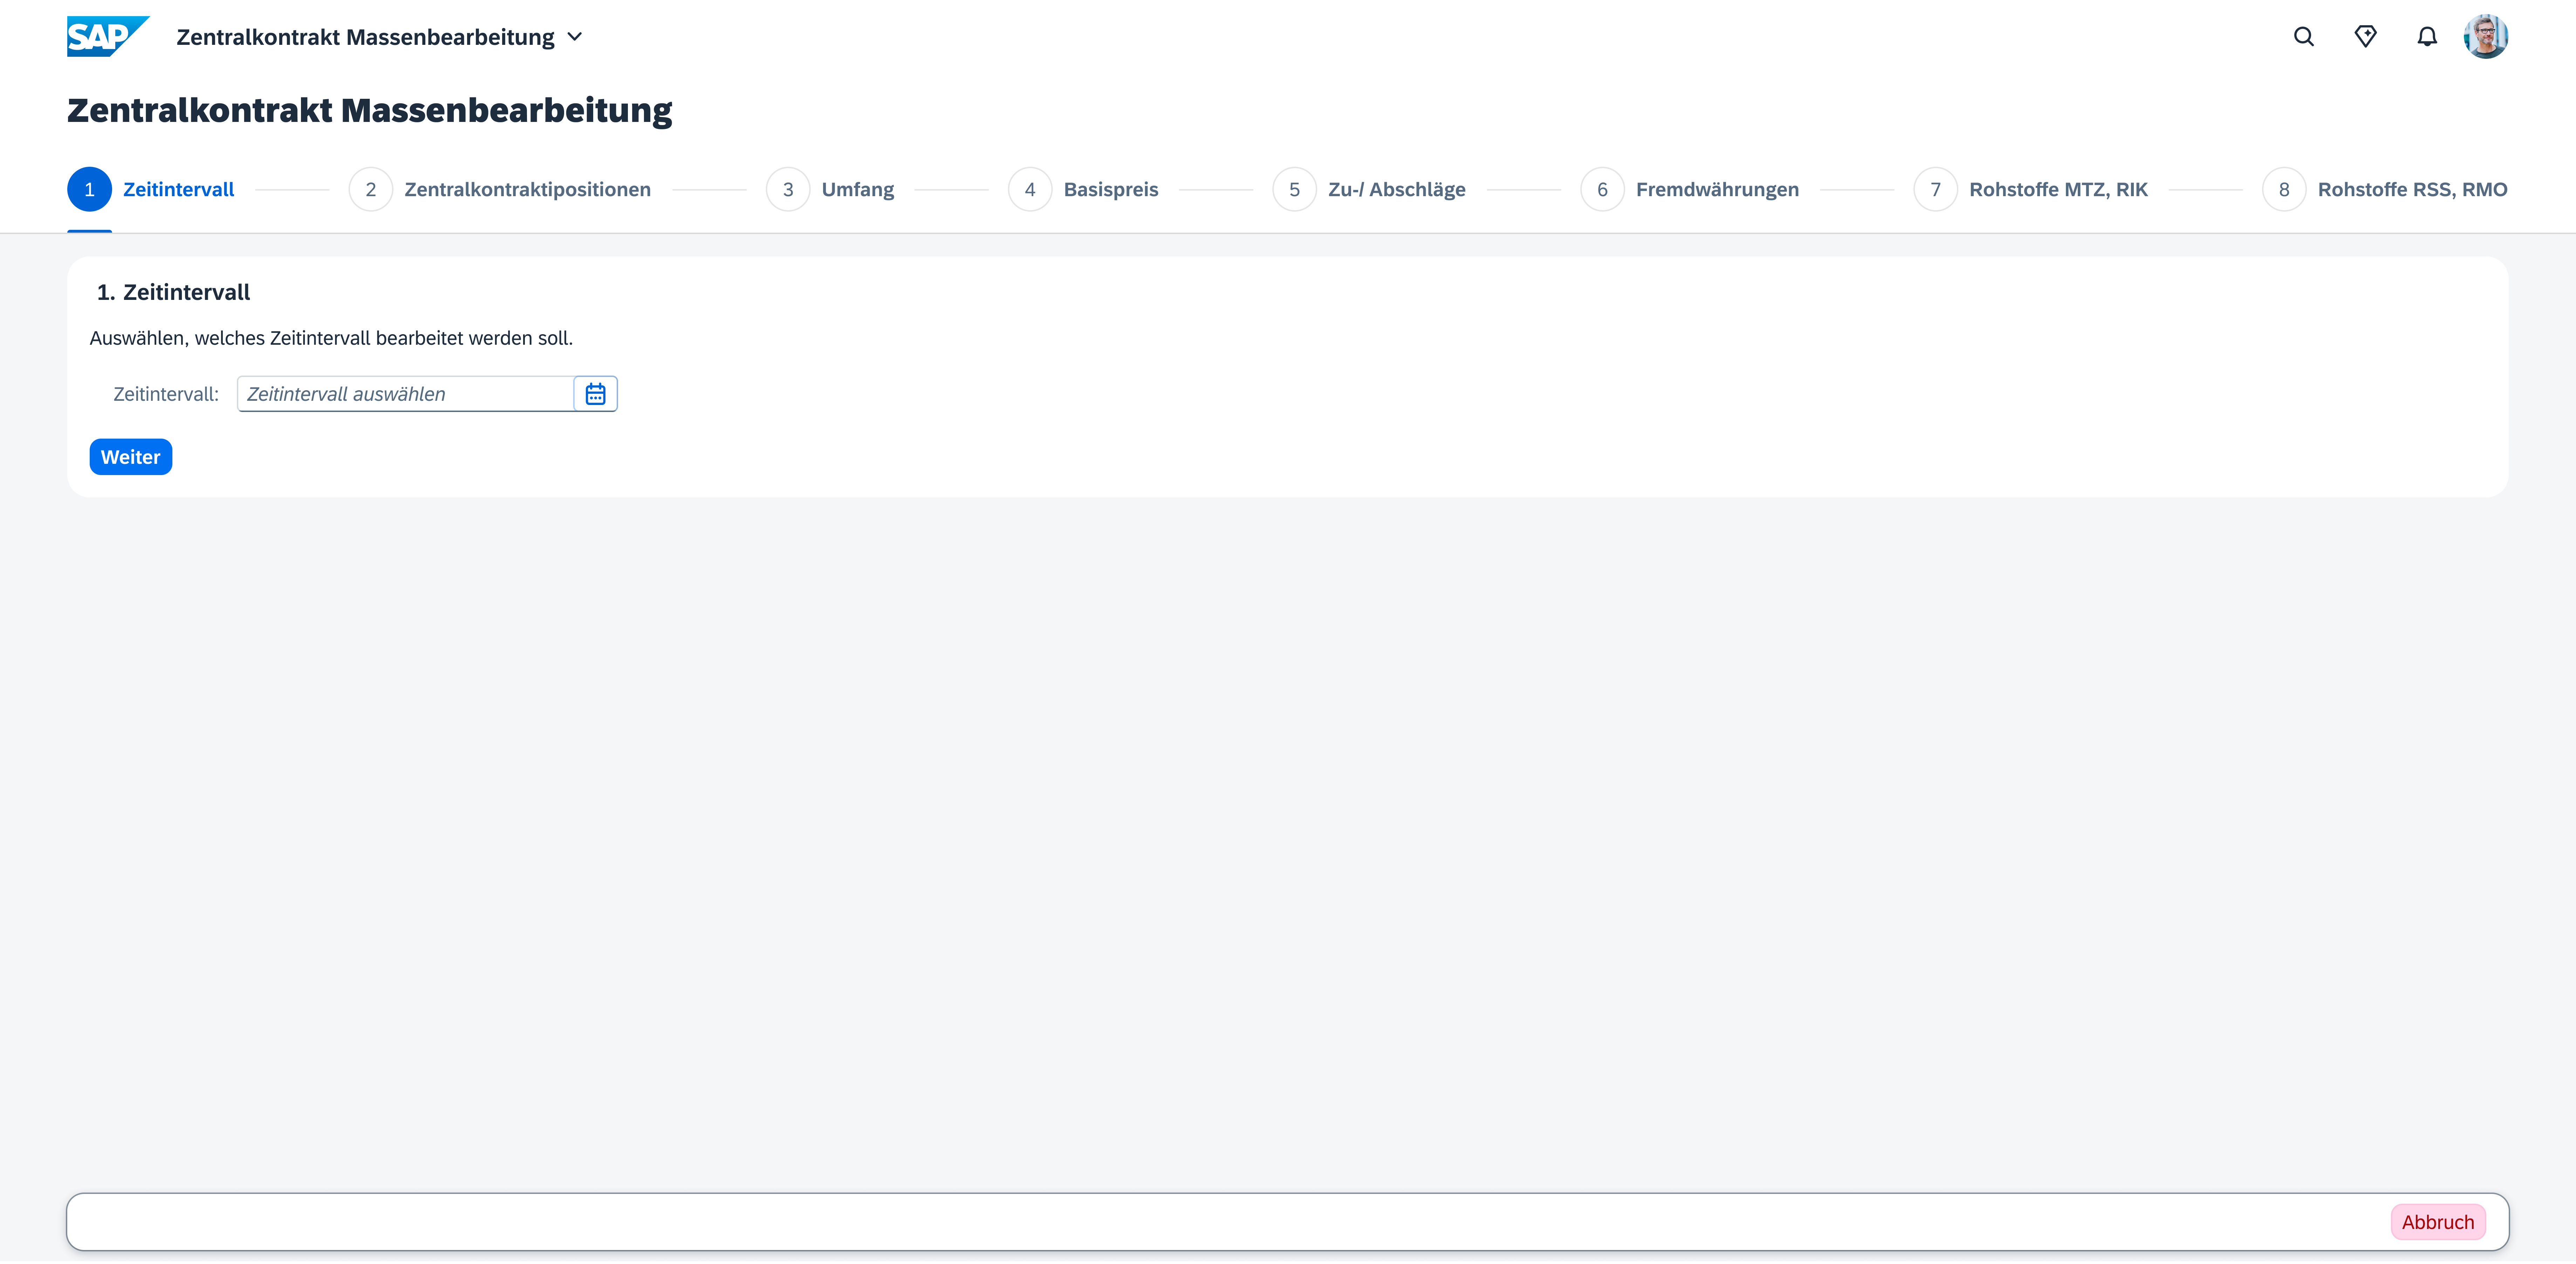
\includegraphics[height=4.76cm]{Bilder/Praxisteil-KL-Schritt-1.png}
    \caption[Massenbearbeitung Central Contracts, Auswahl des Zeitintervalls]{Massenbearbeitung Central Contracts, Auswahl des Zeitintervalls. Eigene Darstellung}
    \label{fig:Central_Contract_Process3}
\end{figure}

asd123456789

%-> Entwicklung einer Fiori-App, über die durch API's die Daten nach der Vorstellung des Kunden im System gepflegt werden können, diese Lösung hätte aber einen enorm hohen Aufwand

\section{Evaluation der verschiedenen Lösungsansätze}

-> Nutzwertanalyse (siehe 1.4)